\documentclass[../poma-notes.tex]{subfiles}

\begin{document}

\subsection*{Cauchy Sequences}

\begin{definition}
  A sequence $\{p_n\}$ in a metric space $X$ is said to be a \textit{Cauchy} sequence if for every $\epsilon > 0$
  there is an integer $N$ such that $d(p_n, p_m) < \epsilon$ if $n \ge N$ and $m \ge N$.
\end{definition}

\begin{anote}
  度量空间 $X$ 中的序列 $\{p_n\}$ 叫做 \textbf{柯西序列 Cauchy},如果对于任何 $\epsilon > 0$ 存在正整数 $N$,
  只要 $m, n \ge N$ 就有 $d(p_n,p_m) < \epsilon$。根据 Wikipedia:
  \begin{figure}[h]
    \centering
    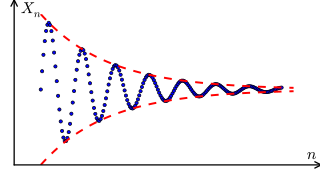
\includegraphics[width=0.5\textwidth]{\subfix{../images/Cauchy_sequence.png}}\par
    一个柯西序列 $\{x_n\}$ 相对于 $n$ 的绘图(蓝色)。如果包含这个序列的空间是完备的,则这个序列的有一个极限。
  \end{figure}

  \begin{figure}[h]
    \centering
    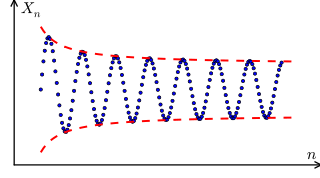
\includegraphics[width=0.5\textwidth]{\subfix{../images/Non_Cauchy_sequence.png}}\par
    一个非柯西序列。这个序列的元素不能随着序列前进而相互靠近。
  \end{figure}
\end{anote}

\begin{definition}
  Let $E$ be a nonempty subset of a metric space $X$, and let $S$ be the set of all real numbers of the form $d(p,q)$,
  with $p \in E$ and $q \in E$. The sup of $S$ is called the \textit{diameter} of $E$.
\end{definition}

如果 $\{p_n\}$ 是 $X$ 中的一个序列,且如果 $E_n$ 包含所有点 $p_N, p_{N+1}, p_{N+2}, \dots$,那么从前两个定义中可以清楚的得到
$\{p_n\}$ 是一个\textbf{柯西序列} 当且仅当
\[\lim_{N \to \infty} diam\ E_N = 0\]

\anote 设 $E$ 是度量空间 $X$ 中的非空子集,又设 $S$ 是一切形式为 $d(p,q)$ 的实数集,$p,q \in E$。$\sup S$ 叫做 $E$ 的直径,
记为 $diam\ E$。

\begin{theorem}
  \begin{enumerate}[label=(\alph*)]
    \item If $\overline{E}$ is the closure of a set $E$ in a metric space $X$, then
          \[diam\ \overline{E} = diam\ E.\]
    \item If $K_n$ is a sequence of compact sets in $X$ such that $K_n \supset K_{n+1} (n=1,2,3,\dots)$ and if
          \[\lim_{n \to \infty} diam\ K_n = 0,\]
          then $\bigcap_1^{\infty} K_n$ consists of exactly one point.
  \end{enumerate}
\end{theorem}

\begin{proof}
  \begin{enumerate}[label=(\alph*)]
    \item 因为 $E \subset \overline{E}$,那么可以清楚的知道
          \[diam\ E \le diam\ \overline{E}\]

          选取 $\epsilon > 0$,$p \in \overline{E}, q \in \overline{E}$。根据 $\overline{E}$ 的定义,$E$ 中存在点 $p'$,$q‘$,
          满足 $d(p,p') < \epsilon,\ d(q,q') < \epsilon$。因此
          \begin{align*}
            \mathcal{} d(p,q) & \le d(p,p') + d(p',q') + d(q',q) \\
                              & < 2\epsilon + d(p',q')           \\
                              & \le 2\epsilon + diam\ E.
          \end{align*}
          它遵循
          \[diam\ \overline{E} \le 2\epsilon + diam\ E,\]
          且因为 $\epsilon$ 是随机的,(a) 则被证明。
    \item 令 $K = \bigcap_1^{\infty} K_n$。根据 Theorem 2.36,$K$ 为非空。如果 $K$ 包含一个以上的点,那么 $diam\ K > 0$。
          但是对于每个 $n$ 而言,$K_n \supset K$,所以 $diam\ K_n \ge diam\ K$。这与假设的 $diam\ K_n \to 0$ 相悖。
  \end{enumerate}
\end{proof}

\begin{anote}
  \begin{enumerate*}[label=(\alph*)]
    \item 如果 $E$ 是度量空间 $X$ 中的集,那么闭包满足 $diam\ \overline{E} = diam\ E$;
    \item 如果 $\{K_n\}$ 是 $X$ 中的紧集的序列,且 $K_n \supset K_{n+1}$ 又若 $\lim_{n \to \infty} diam\ K_n = 0$,
          那么 $\bigcap_1^{\infty} K_n$ 由一个点组成。
  \end{enumerate*}
\end{anote}

\end{document}
